\documentclass[sigconf]{acmart}

\usepackage[utf8]{inputenc}
\usepackage{booktabs} % For formal tables
\usepackage{algorithmicx}
\usepackage{algpseudocode}
\usepackage{algorithm}
\usepackage[inline]{enumitem}

%\usepackage{todonotes}
\usepackage{graphicx}
\graphicspath{figures}
\usepackage{svg}

\def\xcolorversion{2.00}
\def\xkeyvalversion{1.8}

\usepackage{pgf}
\usepackage{tikz}
\usetikzlibrary{arrows,shapes,snakes,automata,backgrounds,petri}

\newcommand\note[2]{{\color{#1}#2}}
\newcommand\todo[1]{{\note{red}{TODO: #1}}}

\newcommand*{\fullref}[1]{\hyperref[{#1}]{\autoref*{#1} (\nameref*{#1})}} % One single link

% Adds a "given" symbol (vertical bar) that rescales in height (like \left and \right)
\usepackage{mathtools}
\newcommand\givenbase[1][]{\:#1\lvert\:}
\let\given\givenbase
\newcommand\sgiven{\givenbase[\delimsize]}
\DeclarePairedDelimiterX\Basics[1](){\let\given\sgiven #1}
\newcommand\Average{E\Basics}

\makeatletter
\newcommand{\StateIndent}[1][3]{%
  \setlength\@tempdima{\algorithmicindent}%
  \Statex\hskip\dimexpr#1\@tempdima\relax}
\algdef{S}[WHILE]{WhileNoDo}[1]{\algorithmicwhile\ #1}%
\makeatother

\newcommand{\algorithmautorefname}{Algorithm}

% Copyright
%\setcopyright{none}
%\setcopyright{acmcopyright}
%\setcopyright{acmlicensed}
\setcopyright{rightsretained}
%\setcopyright{usgov}
%\setcopyright{usgovmixed}
%\setcopyright{cagov}
%\setcopyright{cagovmixed}

% DOI
\acmDOI{10.475/123_4}

% ISBN
\acmISBN{123-4567-24-567/08/06}

%Conference
\acmConference[WOODSTOCK'97]{ACM Woodstock conference}{July 1997}{El
  Paso, Texas USA} 
\acmYear{2017}
\copyrightyear{2017}

\acmPrice{15.00}


\begin{document}
\title{Let's play congestion control}
\titlenote{Produces the permission block, and
  copyright information}
\subtitle{Extended Abstract}
\subtitlenote{The full version of the author's guide is available as
  \texttt{acmart.pdf} document}

\author{Maximilian Bachl} 
\affiliation{%
 \institution{Institute of Telecommunications}
 \streetaddress{Gußhausstraße 25}
 \postcode{1040}
 \city{Vienna} 
 \country{Austria}}
\email{maximilian.bachl@tuwien.ac.at}

\author{Tanja Zseby} 
\affiliation{%
 \institution{Institute of Telecommunications}
 \streetaddress{Gußhausstraße 25}
 \postcode{1040}
 \city{Vienna} 
 \country{Austria}}
\email{tanja.zseby@tuwien.ac.at}

\author{Joachim Fabini} 
\affiliation{%
 \institution{Institute of Telecommunications}
 \streetaddress{Gußhausstraße 25}
 \postcode{1040}
 \city{Vienna} 
 \country{Austria}}
\email{joachim.fabini@tuwien.ac.at}

% The default list of authors is too long for headers}
\renewcommand{\shortauthors}{Bachl, Zseby, Fabini}

\begin{abstract}
This paper proposes a novel method of Congestion Control that uses on-line Reinforcement Learning (RL) to maintain the optimum congestion window with respect to a given utility function. 

To this end we use a neural network based approach that can be initialized with a previously trained neural network or with random weights (without any prior knowledge). As in congestion control the rewards used in the learning process naturally come delayed and bit by bit, we propose a novel formulation of reinforcement learning that allows us to deal with delayed and partial rewards.

We show that our method converges to a stable, close-to-optimum solution within the order of minutes and then commonly outperforms existing congestion control algorithms in typical networks. Thus, for the first time, we demonstrate that ANN based Reinforcement Learning without any preknowledge can feasibly be done on-line and can compete with hand-crafted solutions given long enough episodes. 

\end{abstract}

%
% The code below should be generated by the tool at
% http://dl.acm.org/ccs.cfm
% Please copy and paste the code instead of the example below. 
%
\begin{CCSXML}
<ccs2012>
<concept>
<concept_id>10003033.10003039.10003048</concept_id>
<concept_desc>Networks~Transport protocols</concept_desc>
<concept_significance>500</concept_significance>
</concept>
<concept>
<concept_id>10003752.10010070.10010071.10010261.10010275</concept_id>
<concept_desc>Theory of computation~Multi-agent reinforcement learning</concept_desc>
<concept_significance>500</concept_significance>
</concept>
<concept>
<concept_id>10010520.10010521.10010542.10010294</concept_id>
<concept_desc>Computer systems organization~Neural networks</concept_desc>
<concept_significance>300</concept_significance>
</concept>
</ccs2012>
\end{CCSXML}

\ccsdesc[500]{Networks~Transport protocols}
\ccsdesc[500]{Theory of computation~Multi-agent reinforcement learning}
\ccsdesc[300]{Computer systems organization~Neural networks}

\keywords{congestion control, machine learning, reinforcement learning, artificial neural networks}

\settopmatter{printfolios=true}

\maketitle%

\section{Introduction}

Recent advances in neural network based Reinforcement Learning (RL) for the purpose of playing video games raise the question if it is also possible to formulate sending Internet data in a fashion similar to a video game. The rules of the ``Game of Congestion Control'' can be summarized approximately as follows: Each player wants to send \begin{enumerate*}
\item as many packets as possible
\item with as little delay as possible
\item while losing as few packets as possible
\end{enumerate*}. As, for instance, for some applications overall throughput is more important than little packet loss, each application can define its preference using a custom utility function. Clearly, it is also desirable from an overall point of view that all participating players play the game in a way that does not give them an unfair advantage over others. When several players (from now on called senders) share an Internet link under the same conditions, they should receive an equal share of the reward. 

When performing Congestion Control (CG) \todo{What should be capitalized and what shouldn't? Capitalize RL, CG, ANN?}, each sender uses a set of observed environment conditions to determine what action he should take to maximize his reward in the future. The environment conditions can be any metrics that the sender can obtain from the network, for example the mean round-trip time of the last received packets, the packet loss rate etc. An action is a change to the sending rate: For example, if a sender perceives an increase in the loss rate it might be advisable to lower the sending rate. 

From this formulation of Congestion Control, one can observe a couple of unique features of the problem that seem to prohibit the use of RL: \begin{itemize}
\item When playing a video game, if one pushes a button, one can see the consequences of an action immediately. However, in Congestion Control, the rewards are always \textbf{delayed} by one round-trip time.
\item Due to the delay, by the time an action receives its reward, probably other actions have already been carried out in the mean time. Thus, contrary to classical RL, \textbf{action and rewards are out of sync}. 
\item \textbf{Actions and rewards are not atomic}: If an action causes three packets to be sent, we consider these three packets being sent three \textit{partial actions}. In case these packets are transmitted correctly, the receiver will send three acknowledgements. Each of these acknowledgements is a \textit{partial reward} that already unveils new information on the current state of the network and enables the sender to take an action based on this new information. However, only if all partial rewards have been received, the sender can assemble the overall reward of the corresponding action and can perform an update of the underlying RL logic. 
\end{itemize}

To address these problems, we develop a new formulation of RL called \textit{Partial Action Learning} (PAL). PAL is a superset of Reinforcement Learning: If one uses PAL for a learning problem without delay, asynchronicity and partial actions/partial rewards, one gets classical RL.

While using PAL to train an optimum congestion control for a specific range of network scenarios in an off-line fashion is possible, it is something that has already been done previously in an approach called \textit{Remy} \citep{winstein_tcp_2013}. The only seizable advantage that PAL could provide here is increased training speed. Thus we want to show that it is  not only possible to learn congestion control by using machine learning but that it is even possible to do so on-line and without any preknowledge about the network environment.

Using a utility function that encourages high throughput and discourages packet loss (adapted from \citep{dong_pcc:_2015}) we see that our machine learning based approach can learn congestion control that maximizes this objective given a couple of minutes of time (without any pre-training) \ref{fig:demo}, which -- to our knowledge -- is the first demonstration that neural network based on-line reinforcement learning is possible. 

\begin{figure}
\begin{minipage}{\columnwidth}
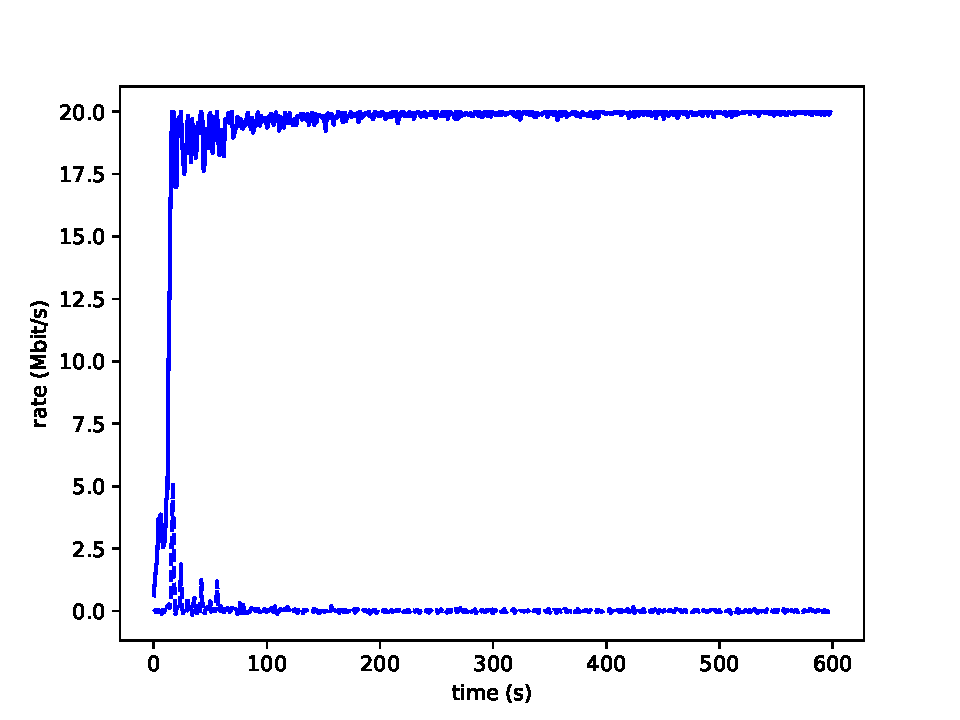
\includegraphics[width=\columnwidth]{figures/1_4}
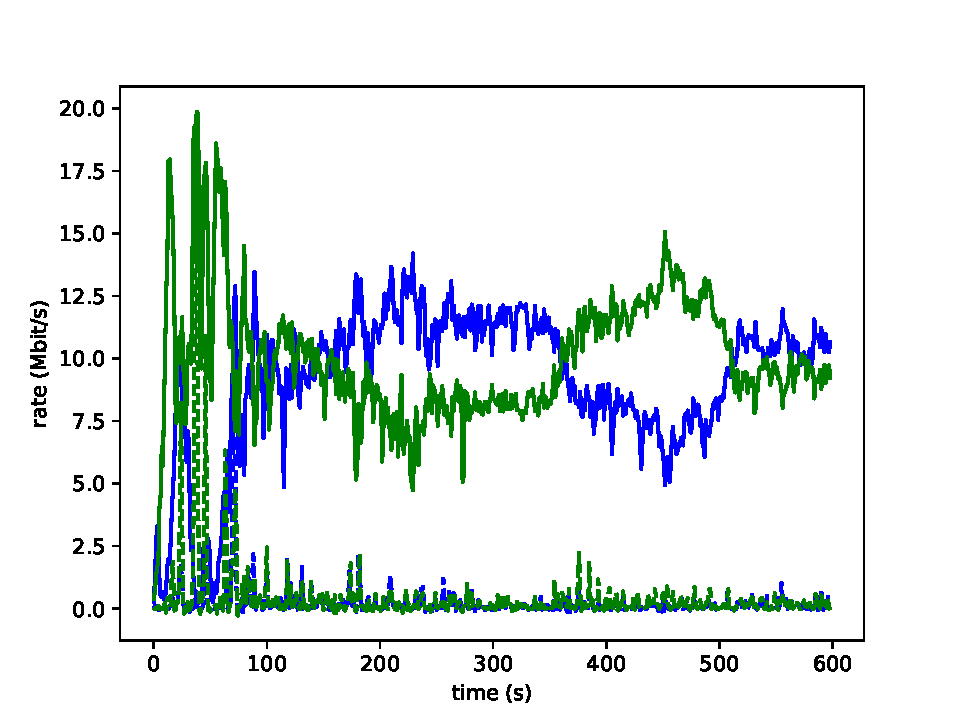
\includegraphics[width=\columnwidth]{figures/2_2}
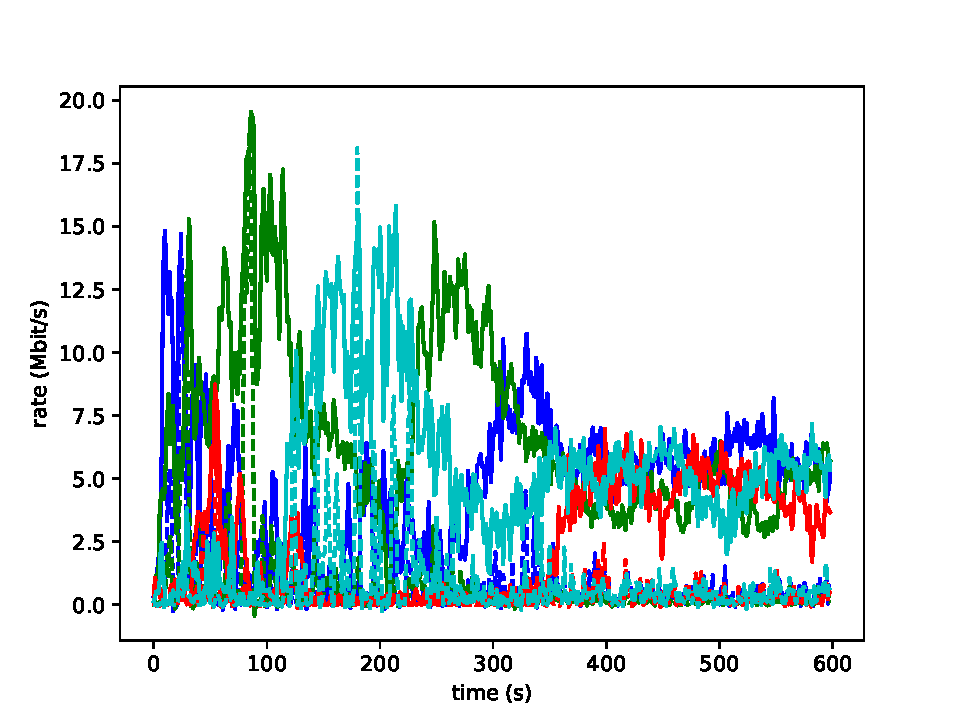
\includegraphics[width=\columnwidth]{figures/4_1}
\caption{\todo{figures don't look that appealing do they?} The throughput (solid line) and the loss rate (dashed line) when sharing a bottleneck link of 20\,Mbit/s with a two-way end-to-end delay of 50\,ms and a very small buffer of $\frac{1}{10}$ bandwidth delay product between 1, 2 and 4 senders (from top to bottom). One can see that the time to convergence increases as the number of senders increases, which is caused by the fact that the more senders use the link, the fewer packets each sender receives per unit of time for training. Also, the complexity of the learning problem increases with more senders as the environment becomes more dynamic and unpredictable.}
\label{fig:demo}
\end{minipage}
\end{figure}

After having learned how to perform congestion control in a certain network scenario, our approach can compete with established algorithms and achieve superior throughput with packet loss at an average of less than 5\%, while still gradually improving and adapting its way of performing congestion control.

\section{Related Work}

\subsection{Congestion Control}

Congestion control has been implemented in TCP since the 1980s as a series of congestion collapses dramatically decreased applications' throughput in the Internet, which lead to the development of the Tahoe and Reno algorithms \cite{jacobson_congestion_1988}. These approaches as well as most others maintain a congestion window which stands for the maximum amount of data that are allowed to be traveling in the network without having been acknowledged by the receiver. In general, successful transmission and acknowledgement of data leads to the congestion window being increased while packet loss (or an increase in delay as in the Vegas algorithm \cite{brakmo_tcp_1995} \todo{How much detail is necessary in the related work section?}) lead to the congestion window being lowered according to a set of fixed rules. Algorithms such as Cubic and Compound \cite{ha_cubic:_2008, tan_compound_2006} improve congestion control specifically with respect to so-called long fat networks with a high round-trip time and bandwidth. Proportional rate reduction \cite{dukkipati_proportional_2011} aims to make the reduction of the rate that occurs in case of congestion more smooth and steady in time to avoid the bursty behavior that occurred upon loss in previous TCP congestion control variants. On the other hand, BBR \cite{cardwell_bbr:_2016} does not use a set of fixed rules such as previous congestion control algorithms but instead estimates a model of the network path by using measurements of RTT and throughput and then adjusts its sending rate so that it uses the maximum bandwidth according to its network model while trying not to fill up queues. A similar approach is PCC \cite{dong_pcc:_2015}, which also uses measurements to find an optimum sending rate with respect to a defined utility function (e.g. maximizing throughput while minimizing packet loss). However, PCC doesn't maintain a congestion window but instead modulates the sending rate. 

Besides the aforementioned human-designed algorithms there have been attempts to use machine learning to improve congestion control. \citet{geurts_machine_2004} train a classifier off-line to determine whether packet loss is caused by congestion or by the link layer. If it is caused by the link layer, TCP does not alter the window. Otherwise -- if a packet was lost due to congestion according to the classifier -- it uses a traditional TCP congestion control algorithm. \citet{winstein_tcp_2013} train a machine learning solution called \textit{Remy} that finds an optimum congestion control for a given range of a range of network parameters. For instance, one could find an optimum congestion control for networks with a RTT of 50-100\,ms and link speeds of 100-500\,Mbit/s. After a lengthy training procedure Remy finds an optimum congestion control algorithm for the specified networks on a per acknowledgement basis. 

Our goal is to find an optimum congestion control algorithm on a per acknowledgement basis similar to Remy that, however, can be trained on-line.  Such a solution could be used in a purely on-line fashion, in a off-line fashion like Remy or a combination of both: One pre-trains a generic congestion control algorithm that works reasonably well for every network that then gets refined during on-line training according to the current network circumstances. 

To this end we use Partial Action Learning which is based on the Asynchronous Advantage Actor Critic framework \cite{mnih_asynchronous_2016}, which has been demonstrated to be able to learn to play a wide range of video games and commonly outperform human players. In particular it is a good choice for congestion control as it can be easily adapted to a wide range of problems and has been proven to deliver good performance. Furthermore, as we will show, it is conceptually possible to use it for on-line training although -- to our knowledge -- this has not been done until now. 

\subsection{Actor Critic Learning}
\label{subsec:ac}

The \textit{Partial Action Learning} (PAL) (see \ref{subsec:pal}) framework is based on the Actor Critic framework for neural networks proposed by \citet{mnih_asynchronous_2016}, which we outline in this section. 

There are two neural networks, the Actor Network and the Value Network (the Critic part in the abbreviation stands for the Value Network). Given a state, the Actor Network outputs what it deems to be the optimum action to perform in that certain state. The Value Network estimates what long-term reward can be expected in this state. So an action is considered good if it achieved a long-term reward that is higher than the long-term reward expected by the Value Network and it is considered bad if the reward was lower than expected. The long-term reward is implemented as an exponentially weighted moving average of future rewards. So if a high reward can be achieved right now this is more favorable than if it can be achieved in the future. However it can also be beneficial to get a low reward now and instead get a very large one in the future. 

\subsubsection{Value Network}
\label{subsubsec:genericvalue}

The Value Network outputs the expected long-term reward $V(s_{t}; \theta_\text{v})$ given a state $s_t$ at time step $t$ and the parameters (neural network weights) of the value network $\theta_v$.

With $r_t$ being the reward that was received at time $t$ and $\gamma$ being a factor with $0 < \gamma \leq 1$, which stands for the influence that future reward has on the moving average, we define the expected long-term reward as 
\begin{align*}
R_t = \gamma r_{t} + (1-\gamma) R_{t+1} ,
%R_t = \left(\left(\sum_{i=0}^{k-1} \gamma^ir_{t+i}\right) + \gamma^k V(s_{t+k}; \theta_\text{v})\right)\left( 1-\gamma \right),
\end{align*}

One can see that to compute $R_t$ at time step $t$ one has to look infinitely far in the future to get all future rewards needed to accurately computer the exponentially weighted moving average at time step $t$. Thus, one usually only carries out $t_\text{max}$ steps (for example 20) and then uses an estimation of $R_{t_\text{max}+1}$ provided by the value network as the continuation \todo{Clearer than before?}. The only exception from this is when the task to carry out is over before reaching $t_\text{max}$. In this case, one can either use a prediction from the value network as usually or simply let the moving average end without continuation (ignoring the term weighted with $(\gamma-1)$ at the last step). 

%where $k$ is upper-bounded by $t_\text{max}$ ($t_\text{max}$ is a fixed hyperparameter that indicates how many rewards should be received before updating the neural network). So $R_t$ is the value of the exponentially weighted average of future rewards at time step $t$. In practice this means that we collect $t_\text{max}$ rewards, compute the expected long-term reward starting at each time step, update the neural network and start the same procedure again. 

%\todo{Explanation not so clear?}

The loss function (not in the sense of packet loss but in the sense of the loss of a machine learning problem), which the value network tries to minimize at each time step, is the square of the difference of the actual long-term reward received and the expected long-term reward
\begin{align*}
l_{\text{v},t} = \left(R_t - V(s_t; \theta_\text{v})\right)^2.
\end{align*}

\subsubsection{Actor Network}
\label{subsubsec:genericactor}

The Actor Network outputs a probability distribution from which the action $a_t$ at time step $t$ is randomly sampled. We use the mean $\mu$ and the standard deviation $\sigma$, to parametrize a normal distribution. The main idea is that the network learns to output the right mean at the right time step to maximize the future reward and that it uses the standard deviation to try out new actions, which could yield a better than expected reward. 

With $v_t$ being the value that the value network estimated as the future reward given the current state $s_t$ at time step $t$ ($v_t$ is just an abbreviation for $V(s_t; \theta_\text{v})$) and $\theta_a$ the parameters of the actor network and with $\beta$ being a factor that specifies the importance of the entropy $H$, $\pi$ designating the probability density function, meaning that $\pi\left( a_t \given s_t; \theta_\text{a} \right)$ is the value of the probability density function of taking action $a_t$ in state $s_t$ with the current weights of the actor network $\theta_\text{a}$, we define the loss that the actor network aims to minimize as follows:
\begin{align*}
l_{\text{a},t} =& -\log \left( \pi\left( a_t \given s_t; \theta_\text{a} \right)\right)\left( R_t - v_t \right)\\ 
&- \beta H\left( \pi\left( s_t; \theta_a \right)\right).
\end{align*}

\section{Method}
\subsection{Partial Action Learning}
\label{subsec:pal}

The key difference between PAL and previous approaches to Reinforcement Learning is that in classical Reinforcement Learning, an action is always followed by a reward and a reward is always followed by a action. In our proposed concept, however, it is possible to take new actions while previous actions haven't received their rewards yet.

Another major difference in PAL is that one action generates a number of partial actions ($\geq 0$) (see \autoref{fig:pal}). Each partial action generates feedback upon interacting with the environment. Upon receiving feedback for a partial action, the agent determines the current state and triggers a new action. When all feedbacks of one action were received, the agent combines them to form the reward and updates the value and actor networks.

In \autoref{alg:pal} we show the code that runs in each of the agents (in the congestion control scenario, one agent corresponds to a sender). It is possible to have several agents which share a set of weights but one can also use separate weights for each agent, which is more realistic in case of congestion control in the Internet, as different senders cannot easily share a set of neural network weights over the Internet.

\begin{figure}
\begin{minipage}{\columnwidth}
\includesvg{Reinforcement_learning_diagram}
\caption{The classical Reinforcement Learning approach.\protect\footnote{adapted from \url{https://upload.wikimedia.org/wikipedia/commons/1/1b/Reinforcement_learning_diagram.svg}}}
\label{fig:reinforcement}
\end{minipage}
\end{figure}

\begin{figure}
\begin{minipage}{\columnwidth}
\includesvg{Reinforcement_learning_diagram_PAL}
\caption{Partial Action Learning: An action consists of zero or more partial actions which trigger feedback upon interacting with the environment. Each feedback updates the state. The value and actor networks are updated upon receiving all feedback of one action.\protect\footnote{adapted from \url{https://upload.wikimedia.org/wikipedia/commons/1/1b/Reinforcement_learning_diagram.svg}}}
\label{fig:pal}
\end{minipage}
\end{figure}

\subsection{Congestion Control specifics}

\begin{figure}

\newcommand{\nodedistance}{2}
\newcommand{\nd}[1]{\numexpr #1 * \nodedistance \relax}

\centering
\begin{tikzpicture}[node distance=\nodedistance,>=stealth',bend angle=45,auto]

  \tikzstyle{place}=[circle,thick,draw=blue!75,fill=blue!20,minimum size=6mm]
  \tikzstyle{transition}=[rectangle,thick,draw=black!75,
  			  fill=black!20,minimum size=4mm]

%  \tikzstyle{every label}=[blue!75]

  \begin{scope}
    \node [place,tokens=1] (s1) at (\nd{0}, \nd{1}) [label={[align=center]left:Receive\\ feedback}] {};
    \node [place] (s2) at (\nd{1}, \nd{2}) [label={[align=center]above:Received\\ ACK}] {};
    \node [place] (s3) at (\nd{2}, \nd{1}) [label={[align=center]right:Packets\\ in the\\ network}] {};
    \node [place] (s4) at (\nd{1}, \nd{0}) [label={[align=center]below:Open congestion\\ window (cwnd)}] {};      

    \node [transition] (e1) at (\nd{0}, \nd{0}) [label=left:Take action] {}
      edge [post] node {$a$}(s4)
      edge [pre] node {1} (s1);    
     
    \node [transition] (e2) at (\nd{2}, \nd{0}) [label={[align=center]right:Send\\ packet}] {}
      edge [pre] node {1} (s4)
      edge [post] node {1} (s3);

    \node [transition] (e3) at (\nd{2}, \nd{2}) [label={[align=center]right:Receive\\ ACK}] {}
      edge [pre] node {1} (s3)
      edge [post] node {1} (s2);

    \node [transition] (e4) at (\nd{1}, \nd{1}) [label={[align=center]left:Update\\open\\cwnd}] {}
      edge [pre] node {1} (s2)
      edge [post] node {1} (s4);
      
    \node [transition] (e5) at (\nd{0}, \nd{2}) [label={[align=center]left:Received\\ feedback}] {}
      edge [pre] node {1} (s2)
      edge [post] node {1} (s1);

  \end{scope}

\end{tikzpicture}

\caption{A petri net describing the congestion control mechanism. We start with one token in the state \textit{Received feedback}, which means that we can take an action right in the beginning. The concept is the following: If there is at least one token in the \textit{Open congestion window}, send a packet. The token goes to the network and after some time the acknowledgement (or timeout if the packet gets lost) for the packet is received in the \textit{Received ACK} state. From here one token goes to the \textit{Open congestion window} meaning that when we get an ACK (or timeout) we can send another packet (The \textit{Open congestion window} signifies the congestion window minus the packets that are currently unacknowledged.). Furthermore the state \textit{Received feedback} receives a token upon receiving an ACK/timeout. \textit{Take action} adds \textit{a} tokens to the \textit{Open congestion window}, where $a$ is a real number (possibly also negative); thus in each state there can also be a real number of tokens (e.g.~ 2.34 tokens are possible in the \textit{Open congestion window}). However, we define that the congestion window can never be smaller than 1 (This means that the sum of all tokens in the \textit{Open congestion window.}, \textit{Received ACK} and \textit{Packets in the network} states can never be smaller than 1.}
\label{fig:petri}
\end{figure}

The motivation for PAL is that classical Reinforcement Learning assumes that a reward follows an action and vice-versa (see \autoref{fig:reinforcement}). However, in the case of congestion control, it is desirable to perform a new action without having received a reward for the previous action. For example, imagine that we receive two acknowledgements directly after one other. For each of these two acknowledgements an action has to be performed but it does not seem feasible for the second action to wait until the first action has received a reward as it takes one RTT until an acknowledgement (a reward) is received. Thus the Asynchronous Actor Critic framework as described by \cite{mnih_asynchronous_2016} cannot be applied to congestion control as it assumes that actions and rewards are synchronized and so we have to use Partial Action Learning (see \autoref{subsec:pal}). We describe the overall workings of PAL for congestion control using a petri net (see \autoref{fig:petri}).

To use PAL for congestion control we first have to define the correct semantics for this specific use case and we have to explicitly state how the state, reward etc.~are defined. Furthermore, we have to define how the actor and value network explicitely work in case of congestion control. In the following a time step $t$ corresponds to the reception of an acknowledgement. The beginning of the flow, before any packet is sent, corresponds to time step $0$.

\begin{description}
\item[$\textit{s}_\text{t}$] The state  describes the current ``congestion state''. The following features are included in it:
\begin{itemize}
\item the round-trip time of the last packet
\item the current congestion window
\item the time between the last two packets that were sent
\item the time between the last two packets that were received
\item the number of packets that were lost since the last acknowledgement was received
\end{itemize}
Each time an acknowledgement is received, the state is updated and the actor network is asked for the next action.
\item[$\textit{a}_\text{t}$] Based on a given state and the history of previous states (because we use LSTM cells and thus can also consider previous states), the actor network returns an action $a_t$, which is a real number that stands for the change of the congestion window. 
\item[$\textit{r}_\text{t}$] The reward is a tuple of at least one reward metric. 
%These are discussed in more detail in \autoref{subsubsec:value}. 
For each reward metric there is also an output of the value network that predicts the expected long-term average of this reward metric given the current state. 
%\item[$\textit{v}_\text{t}$] The value is a tuple of the expected average reward estimated by the value network (see \autoref{subsubsec:value}) for each of the reward metrics. 
\end{description}

We actually use the following types of reward: 
\begin{description}
\item[$\textit{r}_{\text{packet},t}$] is the number of the packets that the sender sent during time step $t$ and that were not lost (so they were acknowledged at some point by the receiver).
%\item[$\textit{r}_{\text{byte},t}$] is the sum of the bytes of the packets that the sender sent and that were not lost. Example: At time $t'$, three packets were sent with 300, 200, and 1500 bytes each so $\textit{r}_{\text{byte},t'} = 2000$
\item[$\textit{r}_{\text{delay},t}$] is the sum of the round trip times of the packets that the sender sent and that were not lost.
\item[$\textit{r}_{\text{duration},t}$] is the sum of the time between receiving the last packet and receiving this packet (``inter-receive time'') for the packets that the sender sent and that were not lost.
\item[$\textit{r}_{\text{lost},t}$] is the sum of packets that were lost between receiving the last packet and receiving this packet.
\end{description}

%We actually use four moving averages for four different types of reward: 
%\begin{description}
%\item[$\textit{R}_\text{packet}$] is the moving average of the packets that the sender sent and that were not lost (so they were acknowledged at some point by the receiver).
%\item[$\textit{R}_\text{byte}$] is the moving average of the bytes of the packets that the sender sent and that were not lost.
%\item[$\textit{R}_\text{delay}$] is the moving average of the round trip time of the packets that the sender sent and that were not lost.
%\item[$\textit{R}_\text{duration}$] is the moving average of the time between receiving the last packet and receiving this packet (``inter-receive time'') for the packets that the sender sent and that were not lost.
%\end{description}

The overall structure of the neural network for both the value and the actor network is depicted in \autoref{fig:neural_network}.

\begin{figure}

\newcommand{\nodedistance}{1.2}
\newcommand{\neuralnetworkwidth}{32}

\pgfmathsetmacro{\shortside}{sqrt((\nodedistance * \nodedistance ) /2)}
\pgfmathsetmacro{\solutionx}{ \shortside }
\pgfmathsetmacro{\solutiony}{ - (3 * \shortside + 3 * \nodedistance ) }

\pgfmathsetmacro{\solutiondurationx}{ \shortside }
\pgfmathsetmacro{\solutiondurationy}{ - (3 * \shortside + 1 * \nodedistance ) }

\centering
\begin{tikzpicture}[every label/.append style={font=\tiny}, node distance=\nodedistance cm, >=stealth',bend angle=45,auto]

  \tikzstyle{place}=[circle,thick,draw=blue!75,fill=blue!20,minimum size=6mm]
  \tikzstyle{input place}=[circle,thick,draw=olive!75,fill=olive!20,minimum size=6mm]
  \tikzstyle{output place}=[circle,thick,draw=magenta!75,fill=magenta!20,minimum size=6mm]
   \tikzstyle{lstm place}=[circle,thick,draw=red!75,fill=red!20,minimum size=6mm]
   \tikzstyle{softplus place}=[circle,thick,draw=green!75,fill=green!20,minimum size=6mm]

  \tikzstyle{transition}=[rectangle,thick,draw=black!75,
  			  fill=black!20,minimum size=4mm]

%  \tikzstyle{every label}=[blue!75]

  \begin{scope}
    \node [input place] (s1) [label={[align=center]left: State (8)}] {};
    \node [place] (s2) [above right of=s1, label={[align=center]above: Linear}] {};
    
  \path[->] (s1) edge node {} (s2);
    
    \node [lstm place] (s3) [right of=s2, label={[align=center]below: GRU (32)}] {};

  \path[->] (s2) edge node {} (s3); 
  \path[->] (s3) edge [loop above] node {} (s3);   
   
    \node [lstm place] (s4) [right of=s3, label={[align=center]below: GRU (32)}] {};    
    
  \path[->] (s3) edge node {} (s4);
  \path[->] (s4) edge [loop above] node {} (s4);
    
    \node [place] (s7) [right of=s4, label={[align=center]below:{ Linear}}] {};
    
  \path[->] (s4) edge node {} (s7);
    
    \node [output place] (s8) [right of=s7, label={[align=center]below: $\sigma$~(1)}] {};    

  \path[->] (s7) edge node {} (s8);

    \node [place] (s5) [above of=s7, label={[align=center]above: Linear}] {};
    
  \path[->] (s4) edge node {} (s5);

    \node [output place] (s6) [right of=s5, label={[align=center]above: $\mu$ (1)}] {};    
    
  \path[->] (s5) edge node {} (s6);    
    
    \node [place] (s10) [below right of=s1, label={[align=center]below: Linear}] {};
    
  \path[->] (s1) edge node {} (s10);

    
    \node [lstm place] (s11) [right of=s10, label={[align=center]above: GRU (32)}] {};
    
  \path[->] (s10) edge node {} (s11);
  \path[->] (s11) edge [loop below] node {} (s11);

    \node [lstm place] (s12) [right of=s11, label={[align=center]above: GRU (32)}] {};
    
  \path[->] (s11) edge node {} (s12);
  \path[->] (s12) edge [loop below] node {} (s12);
    
    \node [place] (s13) [right of=s12, label={[align=center]above: Linear}] {};
    
  \path[->] (s12) edge node {} (s13);

    \node [output place] (s17) [right of=s13, label={[align=center]above: $V_\text{received}$ (1)}] {};
    
  \path[->] (s13) edge node {} (s17);
%    
%    \node [place] (s15) [below of=s13, label={[align=center]above: Linear}] {};
%    
%  \path[->] (s12) edge node {} (s15);
%
%    \node [output place] (s19) [right of=s15, label={[align=center]above: $V_\text{delay}$ (1)}] {};  
    
%  \path[->] (s15) edge node {} (s19);    
    
    \node [place] (s16) [below of=s13, label={[align=center]below: Linear}] {};
    
  \path[->] (s12) edge node {} (s16);    
    
    \node [output place] (s20) [right of=s16, label={[align=center]below: $V_\text{sent}$ (1)}] {};    

  \path[->] (s16) edge node {} (s20);    
    

    \node [place] (s40) at (\solutiondurationx cm,\solutiondurationy cm) [label={[align=center]below: Linear}] {};

  \path[->] (s1) edge node {} (s40);   

    \node [lstm place] (s41) [right of=s40, label={[align=center]above: GRU (32)}] {};
    
  \path[->] (s40) edge node {} (s41);
  \path[->] (s41) edge [loop below] node {} (s41);

    \node [lstm place] (s42) [right of=s41, label={[align=center]above: GRU (32)}] {};
    
  \path[->] (s41) edge node {} (s42);
  \path[->] (s42) edge [loop below] node {} (s42);
       
    \node [place] (s43) [right of=s42, label={[align=center]above: Linear}] {};
    
  \path[->] (s42) edge node {} (s43);
    
    \node [output place] (s44) [right of=s43, label={[align=center]above: $V_\text{duration}$ (1)}] {};   
    
  \path[->] (s43) edge node {} (s44); 
  
%    \node [place] (s17) [below of=s14, label={[align=center]above: Linear}] {};
%    
%  \path[->] (s12) edge node {} (s17);
%    
%    \node [output place] (s22) [right of=s17, label={[align=center]above: $V_\text{byte}$ (1)}] {};   
%    
%  \path[->] (s17) edge node {} (s22);   

%    \node [place] (s30) at (\solutionx cm,\solutiony cm) [label={[align=center]below: Linear}] {};
%
%  \path[->] (s1) edge node {} (s30);   
%
%    \node [lstm place] (s31) [right of=s30, label={[align=center]above: GRU (\neuralnetworkwidth)}] {};
%    
%  \path[->] (s30) edge node {} (s31);
%  \path[->] (s31) edge [loop below] node {} (s31);
%
%    \node [lstm place] (s32) [right of=s31, label={[align=center]above: GRU (\neuralnetworkwidth)}] {};
%    
%  \path[->] (s31) edge node {} (s32);
%  \path[->] (s32) edge [loop below] node {} (s32);
%    
%    \node [place] (s33) [right of=s32, label={[align=center]above: Linear}] {};
%    
%  \path[->] (s32) edge node {} (s33);
%
%    \node [output place] (s34) [right of=s33, label={[align=center]above: $V_\text{byte}$ (1)}] {};
%    
%  \path[->] (s33) edge node {} (s34);

  \end{scope}

\end{tikzpicture}

\caption{An overview of the complete neural network being used. Ocher stands for the input, blue for linear layers, red for LSTM layers, green for linear layers with a softplus activation function and purple for the outputs of the neural network. The numbers in parentheses next to each label stand for the number of width of that layer (i.e.~the number of neurons except for the inputs and outputs).}
\label{fig:neural_network}
\end{figure}

\subsubsection{Value Network}
\label{subsubsec:value}

In the case of congestion control, the loss function $l_{\text{v},t}$ of the value network is actually the sum of the squares of the difference for each of the expected long-term averages and the empirically found averages for each reward metric:
\begin{align*}
l_{\text{v},t} =& \left(R_{\text{packet},t} - V_\text{packet}(s_t; \theta_\text{v})\right)^2 \\
%&+\left(R_{\text{byte},t} - V_\text{byte}(s_t; \theta_\text{v})\right)^2 \\
&+\left(R_{\text{delay},t} - V_\text{delay}(s_t; \theta_\text{v})\right)^2 \\
&+\left(R_{\text{duration},t} - V_\text{duration}(s_t; \theta_\text{v})\right)^2 \\
&+\left(R_{\text{lost},t} - V_\text{lost}(s_t; \theta_\text{v})\right)^2
\end{align*}

\subsubsection{Actor Network}
\label{subsubsec:actor}

The actor network outputs two parameters: The mean of a normal distribution $\mu$ and its standard deviation $\sigma$. 

Each time an action $a_t$ is requested, it is sampled from the current normal distribution defined by the parameters $\mu$ and $\sigma$.

Then the window is incremented by $a_t$; however, the window can never be smaller than 1. At the beginning of a flow the window starts with 1 as well.

With $H$ being the entropy, the actor network minimizes the loss
%\begin{align*}
%l_{\text{a},t} =& -\log \left( \pi \left( a_t \given s_t ; \theta_\text{a} \right) \right)\\
%&\left( \left(\log\left(\frac{R_{\text{byte},t}}{{R_{\text{duration},t}}}\right) - \log\left(\frac{v_{\text{byte},t}}{{v_{\text{duration},t}}}\right)\right) - \left( \frac{R_{\text{delay},t}}{{R_{\text{packet},t}}}- \frac{v_{\text{delay},t}}{{v_{\text{packet},t}}} \right)\right)\\ 
%&+ \beta H\left( \pi\left( s_t; \theta_a \right)\right).

\begin{align*}
l_{\text{a},t} =& -\log \left( \pi \left( a_t \given s_t ; \theta_\text{a} \right) \right)\\
& \left( U_{\text{measured},t} - U_{\text{expected},t} \right)\\ 
&- \beta H\left( \pi\left( s_t; \theta_a \right)\right)
\end{align*}
where $U$ can be any utility function defined based on some of the reward metrics. In the above formulation, one considers how much better the actual experienced Utility was compared to the expected one. The Utility is formed from the previously defined expected long-term values. 
 
\subsection{Utility function}

As the utility function one can choose an arbitrary function based on the reward metrics previously defined. A safe choice is to use PCC's \citep{dong_pcc:_2015} reward function as its convergence has been previously proven. It is defined as follows:

\begin{align*}
U_t = r_{\text{received},t}\text{Sigmoid}_\alpha\left(\frac{r_{\text{loss},t}}{r_{\text{sent},t}} - 0.05\right) + r_{\text{loss},t}
\end{align*}
where 
\begin{align*}
\text{Sigmoid}_\alpha(x) = \frac{1}{1+e^{\alpha x}},
\end{align*}
$r_\text{received}$ is the actual throughput (in packets per second), $r_\text{loss}$ is the loss rate (in packets per second) and $r_\text{sent}$ is the sending rate (in packets per second). Thus $\frac{r_\text{loss}}{r_\text{sent}}$ is the ratio of data getting lost compared to those being sent, which is a number between 0 and 1.

Intuitively it means that one takes the actual throughput (packets that get received by the receiver and do not get lost) times the sigmoid function of the loss ratio minus 0.05 plus the loss rate. The sigmoid function essentially acts as a cutoff threshold. As soon as the loss rate rises above 5\%, the Sigmoid function decreases very quickly and thus diminishes the Utility. 

It is also possible to set the cutoff threshold to 0, which means that losing packets is heavily punished; or one can increase the threshold to allow for more loss. 

$r_{\text{received},t}$ can be calculated as $\frac{R_\text{packet},t}{R_\text{duration},t}$, $r_{\text{loss},t}$ can be calculated as $\frac{R_\text{lost},t}{R_\text{duration},t}$ and $r_{\text{sent},t}$ can be calculated as $\frac{{R_\text{packet},t} + {R_\text{lost},t}}{R_\text{duration},t}$.

Actually, we assume equally sized packets for all of the above methodology, however, it would also easily be possible to consider the number of bytes per packet as well: One would have to add an additional reward metric of the average number of bytes per packet and as well add one more output to the value network. 

\subsection{Example}

In this section, an example of the overall procedure is outlined. 

\begin{enumerate}
\item Receive an ACK
\item Update the internal state to reflect the information that this ACK provides (for example, the state consists of the round trip time experienced by this packet, the time since we receive the last ACK etc.)
\item Sample an increase for the congestion window from the Actor Network (e.g. $0.24$) and add it to the current congestion window.
\item 
\begin{enumerate}
\item If this was the last ACK, which completes a previous action (e.g. a previous action resulted in $3$ packets being sent; so if this is the ACK for the third (and last) packet of this previous action, we got all the ACKs to compute the reward), combine all partial rewards to form the actual reward for that action. 
\item If we now have $t_\text{max}$ rewards (set to 20) then we also update the neural network. 
\end{enumerate}

\end{enumerate}

\section*{Appendix}

\begin{algorithm}[H]
\caption{Partial Action Learning -- pseudocode for each agent. It is possible that the agents share the global weights $\theta_{\text{a},\text{g}}$ and $\theta_{\text{v},\text{g}}$, which can be reasonable when learning off-line. Otherwise an individual copy of them is kept by each agent. All weights are initialized randomly in the beginning. LSTM cells are used in both the actor and the value network.}
\label{alg:pal}
\begin{algorithmic}[1]
\Loop
	\State $l_\text{actions} \gets  [] $
	\State $l_\text{states} \gets  [] $
	\State $l_\text{values} \gets  [] $
	\State $l_\text{rewards} \gets  [] $
	\State $l_\text{estimatedValues} \gets  [] $
	\State $l_\text{snapshots} \gets  [] $
	\State $l_\text{hiddenStates} \gets  [] $
	\State $t \gets 0$
	\State $s_0 \gets \text{initialState}()$
	\State $h_\text{a} \gets \text{initialHiddenState}()$
	\State $h_\text{v} \gets \text{initialHiddenState}()$
	\State $\theta_\text{a} \gets \theta_{\text{a},\text{g}}$
	\State $\theta_\text{v} \gets \theta_{\text{v},\text{g}}$
	\Repeat
		\State $l_\text{estimatedValues}.\text{append}(V(s_t; \theta_\text{v}))$
		\If{$t \bmod t_\text{max} = 0$}
			\State $\theta_\text{a} \gets \theta_{\text{a},\text{g}}$
			\State $\theta_\text{v} \gets \theta_{\text{v},\text{g}}$
			\State $l_\text{snapshots}.\text{append}((\theta_\text{a}, \theta_\text{v}))$
			\State $l_\text{hiddenStates}.\text{append}((h_\text{a}, h_\text{v}))$
		\EndIf
		\State $l_\text{states}.\text{append}(s_t)$
		\State Sample $a_t$ from the 
		\StateIndent[3] Actor Network's probability distribution
		\State $l_\text{actions}.\text{append}(a_t)$
		\State $l_\text{values}.\text{append}(V(s_t; \theta_\text{v}))$
		\State $l_{\text{partialActions},t} \gets \text{partialActions}(a_t)$
		\ForAll{partial actions $a_{{\text{p},i,t}}$ in $l_{\text{partialActions},t}$}
			\State Take partial action $a_{{\text{p},i,t}}$
		\EndFor
		\State Wait for the next feedback $r_{\text{p},j,t'}$
		\StateIndent[3] where $t' \leq t$ and $0 \leq j \leq\#(l_{\text{partialActions},t'})$
		\If{all feedback of $a_{t'}$ was received}
			\State $r_{t'} \gets \text{reward w.r.t all feedback }r_{\text{p},k,t'}$
					\StateIndent[4] where $0 \leq k \leq\#(l_{\text{partialActions},t'})$
			\State $l_\text{rewards}.\text{append}(r_{t'})$
			\If{$\#\left(l_\text{rewards}\right) > t_\text{max}$ or the episode is over}
				\State \Call{computeGradients}{}
			\EndIf
		\EndIf
		\State Generate $s_{t+1}$ using $r_{\text{p}_{t'}}$
		\State $t \gets t+1$
	\Until{reaching the end the episode}
\EndLoop
%\algstore{palalg}
\end{algorithmic}
\end{algorithm}

\begin{algorithm}[H]
\caption{Partial Action Learning -- procedure which computes and applies the gradients.}
\label{alg:grad}
\begin{algorithmic}[1]%
%\algrestore{palalg}
\Function{computeGradients}{}
	\State $t_\text{end} = \min\left(t_\text{max}, \#\left( l_\text{rewards} \right)\right)$
	\State $\theta_\text{backup} \gets \left(\theta_\text{a}, \theta_\text{v}\right)$
	\State $h_\text{backup} \gets \left(h_\text{a}, h_\text{v}\right)$
	\State $\theta_\text{a}, \theta_\text{v} \gets l_\text{snapshots}[0]$
	\State $h_\text{a}, h_\text{v} \gets l_\text{hiddenStates}[0]$
	\State $R_{i+1} \gets$ last element of $l_\text{estimatedValues}$%
	\For{$i\gets t_\text{end}-1, 0$}
		\State $R_i \gets \left(r_i + \gamma R_{i+1}\right)\left(1-\gamma\right)$
		\State $a \gets l_\text{actions}[i]$
		\State $s \gets l_\text{states}[i]$
		\State $v \gets l_\text{values}[i]$
		\State $d\theta_\text{a} \gets -\frac{\partial\log \left( \pi\left( a \given s; \theta_\text{a} \right)\right)\left(R_i - v\right)}{\partial\theta_a}$
		\StateIndent[4] $-\frac{\partial\beta H\left( \pi\left( s; \theta_a \right)\right)}{\partial\theta_a}$
		\State $d\theta_\text{v} \gets \frac{\partial\left(R_i - v\right)}{\partial\theta_v}$
		\State $\theta_{\text{a},\text{g}} \gets \theta_{\text{a},\text{g}} + d\theta_\text{a}$
		\State $\theta_{\text{v},\text{g}} \gets \theta_{\text{v},\text{g}} + d\theta_\text{v}$
	\EndFor
	\State Remove first $t_\text{end}$ elements from
	\StateIndent[2] $l_\text{actions}$, $l_\text{states}$, $l_\text{values}$, $l_\text{rewards}$, $l_\text{estimatedValues}$
	\State Remove the first element from $l_\text{snapshots}$
	\State Remove the first element from $l_\text{hiddenStates}$
	\State $\theta_\text{a}, \theta_\text{v} = \theta_\text{backup}$
	\State $h_\text{a}, h_\text{v} = h_\text{backup}$
\EndFunction
\end{algorithmic}
\end{algorithm}

%\subsection{Convergence}
%
%We use 
%
%\begin{align*}
%\text{Reward} = \log(\text{throughput}) - \delta\text{delay}
%\end{align*}
%
%as our metric of reward, where $\delta$ is a parameter that allows us to change the importance of the throughput vs.~the delay. We take the logarithm of the throughput to ensure that flows which have small throughput have a higher incentive to increase it as flows which already have a large one (because the derivative of the logarithm decreases with increasing value). We take minus the delay to punish inducing delay. We do not take the logarithm because we think that it is equally bad if a sender behind a satellite connection with a minimum RTT of $500\,$ms adds $1\,$ms of delay as if a sender connected using Ethernet with a minimum RTT of $10\,$ms adds $1\,$ms of delay. 
%
%There are two conditions that we have to take into account to ensure convergence:
%\begin{enumerate}
%\item \begin{align*}
%\left(\frac{\partial}{\partial w}\text{throughput}\right)\left(1\right) > \left(\frac{\partial}{\partial w}\delta\text{delay}\right)\left(1\right)
%\end{align*}
%\item \begin{align*}
%\frac{\partial}{\partial w}\left(\delta\right)
%\end{align*}
%\end{enumerate}
%
%\todo{Finish second constraint for convergence.}
%
%\todo{Add figure to visually explain that}

%\subsection{Convergence}
%
%Assume we have $N$ senders, each with its specific baseline delay (this encompasses all delays excluding only the queueing delay) $d_i$. Each sender keeps a congestion window $b_i$. The link speed at the bottleneck is designated as $c$. 
%
%%We define the excessive window as 
%%\begin{align*}
%%b_\text{excess} = \max\left( \left( \sum_{j=1}^N \frac{b_j}{d_j} \right) - c, 0 \right)
%%\end{align*}
%%and the queueing delay as 
%%\begin{align*}
%%d_q = \frac{b_\text{excess}}{c}.
%%\end{align*}
%
%With $b = (b_i)$ we observe the following relation:
%
%\begin{align*}
%c = \sum_{j=1}^N \frac{b_j}{d_j + d_q(b)}
%\end{align*}
%
%Then we define the utility function for each sender $i$ as
%\begin{align*}
%V_i(b) \coloneqq \begin{cases}
%\log\left(\frac{b_i}{d_i}\right) - \delta_i d_i & \text{if } \sum_{j=1}^N \frac{b_i}{d_i} \leq c\\
%\log\left(\frac{b_i}{d_i + d_q(b)}\right) - \delta_i (d_i + d_q(b)) & \text{otherwise}
%\end{cases}
%\end{align*}
%
%\begin{align*}
%&\log\left(\frac{b_i}{d_i + d_q}\right) - \delta_i (d_i + d_q) \\
%=& \log\left(b_i\right) - \log\left(d_i + d_q\right) - \delta_i (d_i + d_q)
%\end{align*}
%
%\begin{align*}
%\frac{\partial V_i}{\partial b_i} = \begin{cases}
%\frac{1}{b_i} & \text{if } \sum_{j=1}^N \frac{b_i}{d_i} \leq c\\
%\frac{1}{b_i} - \frac{\partial d_q}{\partial b_i}\left(b_i\right)\frac{1}{d_i+d_q\left(b_i\right)} - \delta\frac{\partial d_q}{b_i}\left(b_i\right) & \text{otherwise}
%\end{cases}
%\end{align*}

%\begin{align*}
%G(b) = \begin{pmatrix}
%-\frac{1}{b_1^2} & & \\
%& \ddots & \\
%& & -\frac{1}{b_N^2}
%\end{pmatrix} \text{if } \text{if } \sum_{j=1}^N \frac{b_i}{d_i} \leq c
%\end{align*}

%To show diagonal strict concavity we have to show that d.s.c.~is fulfilled \begin{enumerate*} \item for two distinct points lying in $\sum_{j=1}^N \frac{b_i}{d_i} \leq c$ \item for two distinct points lying in $\sum_{j=1}^N \frac{b_i}{d_i} > c$ and \item when one point is in one part of the function and the other in the other one\end{enumerate*}.
%
%\todo{Insert what d.s.c~actually is and quote Altman's paper}

%\begin{enumerate}
%\item (b^1 - 
%\item
%\item
%\end{enumerate}

%\section{Results}
%
%We train on the following scenario:
% 
%\begin{table}[h]
%\centering
%\begin{tabular}{rll}
%\toprule
%Parameter & Value & Distribution \\
%\midrule
%Two-way propagation delay & $100\,$ms & constant \\
%Bottleneck bandwidth & $3\,$Mbit/s & constant \\
%Number of senders & $2$ & constant \\
%Flow length & $\infty$ & constant \\
%Simulation duration & $50\,$s--$150\,$s & uniform \\
%Buffer size & $\infty$ & constant \\
%Stochastic loss prob. & $0\%$ & constant \\
%\bottomrule
%\end{tabular}
%\caption{The parameters of our very first simple experiment}
%\label{tab:smallexperiment}
%\end{table}
%
%\todo{Insert results when comparing to regular TCP}
 
\bibliographystyle{ACM-Reference-Format}
\bibliography{congestion}

\end{document}
